\section{Nitro Protocol}

Nitro protocol is an extension to Turbo protocol.
In Nitro protocol, the outcome of a channel can be either an allocation or a \textbf{guarantee}.
A guarantee outcome specifies the address of a target allocation channel; the protocol specifies how this guarantee may be used to pay debt on its behalf.
When paying debt, a guarantee can be used to alter the payout priority of the allocation outcome of its target address. 

\begin{tikzpicture}
  \node[semicircle, draw] (upper) at (0,0) {};
  \node[semicircle, draw, rotate=180] (lower) at (0,-1) {};

  \draw[-] (upper.220) to (lower.320);
  \draw[-] (upper.270) to (lower.270);
  \draw[-] (upper.320) to (lower.220);

  \node[semicircle, draw] (upper1) at (1,0) {};
  \node[semicircle, draw, rotate=180] (lower1) at (1,-1) {};

  \draw[-] (upper1.220) to[out=270, in=90] (lower1.270);
  \draw[-] (upper1.270) to[out=270, in=90] (lower1.220);
  \draw[-] (upper1.320) to[out=270, in=90] (lower1.320);

  \node[semicircle, draw, rotate=30] (upper2a) at (2,0) {};
  \node[semicircle, draw, rotate=-30] (upper2b) at (3,0) {};
  \node[semicircle, draw, rotate=180] (lower2) at (2.5,-1) {};

  \draw[-] (upper2a.220) to[out=300, in=90] (lower2.320);
  \draw[-] (upper2a.270) to[out=300, in=90] (lower2.220);
  \draw[-] (upper2a.320) to[out=300, in=90] (lower2.270);

  \draw[-] (upper2b.220) to[out=240, in=90] (lower2.270);
  \draw[-] (upper2b.270) to[out=240, in=90] (lower2.220);
  \draw[-] (upper2b.320) to[out=240, in=90] (lower2.320);
\end{tikzpicture}


We will use the notation $\guar{L}{A_1, A_2, \dots, A_m}$ for a guarantee with target $L$, which prioritizes payouts to $A_1$ above $A_2$, $A_2$ above $A_3$, and so on.
Any addresses which occur in the outcome of $L$ but not in the guarantee are prioritized after $A_m$, in the order they occur in the outcome.
We say a guarantor channel, $G$, which targets an allocation channel, $L$, `can afford $x$ for $A$', if $A$ would receive at least $x$ coins, were the coins currently held in $A$ to be paid out according to $G$'s reprioritization of $L$'s allocation.

Nitro adds the \textbf{claim} operation, $\claim{G}{A}{x}$, to the existing transfer, deposit and withdraw operations.
If $G$ acts as guarantor for $L$ and can afford $x$ for $A$, then $\claim{G}{A}{x}$ has the following three effects:
\begin{itemize}
  \item Reduces the funds held in channel $G$ by $x$.
  \item Increases the funds held in channel $A$ by $x$.
  \item Reduces the amount owed to $A$ in the outcome of $L$ by $x$.
\end{itemize}
Otherwise, the claim operation has no effect.


\begin{tikzpicture}[x=8cm, y=2cm]
  \node[draw=black, rounded corners=0.5cm] (adj0) at (0, 0) {
    \begin{tabular}{c|c|c}
      \multicolumn{3}{c}{\textbf{Adjudicator}} \\
      Address & Balance & Outcome \\
      \hline
      $G$ & 3 & $\guar{L}{\text{Alice}}$\\
      $L$ &  & Bob: 2, Alice: 3 \\
    \end{tabular}
  };

  \node[draw=black, rounded corners=0.5cm] (adj0) at (1, 0) {
    \begin{tabular}{c|c|c}
      \multicolumn{3}{c}{\textbf{Adjudicator}} \\
      Address & Balance & Outcome \\
      \hline
      $G$ &  & $\guar{L}{\text{Alice}}$\\
      $L$ &  & Bob: 2 \\
      Alice & 3 \\
    \end{tabular}
  };

  \node (not0) at (0, -1) { $\adj{\holds{G}{3}{\guar{L}{\text{Alice}}}, \;\holds{L}{}{\alloc{\text{Bob}:2, \text{Alice}:3}}}$ };
  \node (not1) at (1, -1) { $\adj{\holds{G}{}{\guar{L}{\text{Alice}}}, \;\holds{L}{}{\alloc{\text{Bob}:2}}, \;\holds{\text{Alice}}{3}{}}$ };

  \node (diag0) at (0, -2) {
    \begin{tikzpicture}[y=1cm, x=2cm]
      \node[sqadj] (a0) at (0, 0) {};
      \node[circB, label=below:Bob] (p0) at (0, -1) {};
      \draw[->] (a0) edge node[midway, left] { $4$ } (p0);

      \node[sqadj] (a0) at (1, 0) {};
      \node[circAB, label=right:L] (p0) at (1, -1) {};
      \node[circB, label=below:Bob] (p1) at (0.58, -2) {};
      \node[circA, label=below:Alice] (p2) at (1.42, -2) {};


      \draw[->] (a0) edge node[midway, left] { $5$ } (p0);
      \draw[->] (p0) edge node[midway, left] { $2$ } (p1);
      \draw[->] (p0) edge node[midway, left] { $3$ } (p2);

    \end{tikzpicture}
  };

  \node (diag1) at (1, -2) {
    \begin{tikzpicture}[y=1cm, x=2cm]
      \node[sqadj] (a0) at (0, 0) {};
      \node[circB, label=below:Bob] (p0) at (0, -1) {};
      \draw[->] (a0) edge node[midway, left] { $4$ } (p0);

      \node[sqadj] (a1) at (1, 0) {};
      \node[circAB, label=right:L] (pab) at (1, -1) {};
      \node[circB, label=below:Bob] (pabb) at (1, -2) {};
      \draw[->] (a1) edge node[midway, left] { $5$ } (pab);
      \draw[->] (pab) edge node[midway, left] { $2$ } (pabb);

      \node[sqadj] (a2) at (2, 0) {};
      \node[circA, label=below:Alice] (pa) at (2, -1) {};
      \draw[->] (a2) edge node[midway, left] { $3$ } (pa);

    \end{tikzpicture}
  };
\end{tikzpicture}



\begin{example}
  In the following example, we have a guarantor channel, $G$, which holds $5$ coins and guarantees $L$'s allocation, with $B$ as highest priority.
  \begin{multline}
    \claim{G}{B}{5}\adj{\holds{G}{5}{\guar{L}}{B}, \holds{L}{}{\alloc{A: 5, B: 5}}} = \\ \adj{\holds{G}{}{\guar{L}{B}}, \holds{L}{}{\alloc{A: 5}}, \holds{B}{5}{}}
  \end{multline}
  Note that after the claim has gone through, $L$'s debt to $B$ has decreased.
\end{example}

We give a python implementation of an adjudicator implementing the Nitro protocol in the appendix.

\subsection{Virtual Channels}

A virtual channel is a channel between two participants who do not have a shared on-chain deposit, supported through an intermediary.
We will now give the construction for the simplest possible virtual channel, between $A$ and $B$ through a shared intermediary, $I$.
Our starting point for this channel is a pair of ledger channels, $L$ and $L'$, with participants $\{A,I\}$ and $\{B,I\}$ respectively.
\begin{align}
  \adj{\holds{L}{x}{}, \holds{L'}{x}{}}, \; \finalizable{L}{\alloc{A:a, I:b}}{A, I}, \; \finalizable{L'}{\alloc{B: b, I: a}}{B, I} \label{eq:virtual-channel-start-state}
\end{align}
where $x = a + b$.
The participants want to use the existing deposits and ledger channels to fund a virtual channel, $\rchi$, with $x$ coins.

In order to do this the participants will need three additional channels: a joint allocation channel, $J$, with participants $\{A, B, I\}$ and two guarantor channels $G$ and $G'$ which target $J$. The setup is shown in figure \ref{fig:virtual-channel-construction}.

\begin{figure}[ht]
  \centering
  \begin{tikzpicture}
  \node at (0, 0) {
    \begin{tikzpicture}[x=2.4cm, y=1cm, framed, background rectangle/.style={draw=black,dashed, rounded corners}] 

      % Specification of nodes (position, etc.)
      \node (a0) at (0,0) { $\adj{\holds{L}{x}{}, \holds{L'}{x}{}}$ };
      \node (b0) at (-1,-1) { $\finalizable{L}{\alloc{G: x}}{A, I}$ };
      \node (b1) at (1,-1) { $\finalizable{L'}{\alloc{G': x}}{B, I}$ };
      \node (g0) at (-1,-2) { $\finalizable{G}{\guar{J}{\rchi, A, I}}{A, I}$ };
      \node (g1) at (1,-2) { $\finalizable{G'}{\guar{J}{\rchi, B, I}}{B, I}$ };
      \node (j) at (0,-3) { $\finalizable{J}{\alloc{\rchi: x, I: x}}{A,B,I}$ };

      \begin{scope}[-]
        \tikzstyle{every node}=[draw=none,below]
        \draw (a0) to (b0);
        \draw (a0) to (b1);
        \draw (b0) to (g0);
        \draw (b1) to (g1);
        \draw (g0) to (j);
        \draw (g1) to (j);
      \end{scope}
    \end{tikzpicture}
  };

  \node at (7, 0) {
    \begin{tikzpicture}[x=.8cm, y=0.85cm]
      \node[sqadj] (a0) at (-1,0) {};
      \node[sqadj] (a1) at (1,0) {};
      \node[circAI, label=left:$L$] (b0) at (-1,-1) {};
      \node[circBI, label=right:$L'$] (b1) at (1,-1) {};
      \pic (G) at (0, -2.5) {guarantee2};
      \node[circAB, label=below:$\rchi$] (ab) at (-0.7,-4) {};
      \node[circI, label=below:$I$] (i) at (0.7, -4) {};

      \begin{scope}[->]
        \draw (a0) edge node[midway, left] { 10 } (b0);
        \draw (a1) edge node[midway, right] { 10 } (b1);
        \draw (b0) edge node[midway, left] { 10 } (G-G0);
        \draw (b1) edge node[midway, right] { 10 } (G-G1);
        \draw (G-J) edge node[midway, left] { 10 } (ab);
        \draw (G-J) edge node[midway, right] { 10 } (i);
      \end{scope}
    \end{tikzpicture}
  };
\end{tikzpicture}

  \caption{Virtual channel construction}
  \label{fig:virtual-channel-construction}
\end{figure}

We will cover the steps for safely setting up this construction in section \ref{section:open-close-virtual-channel}. 
In the next section, we will explain why this construction can be considered to fund the channel $\rchi$.

\subsection{Offloading Virtual Channels}

Similarly to the method for ledger channel construction, we will show that the virtual channel construction funds $\rchi$ by demonstrating how any one of the participants can offload the channel $\rchi$, thereby converting it to an on-chain channel that holds its own funds.

We will first consider the case where $A$ wishes to offload $\rchi$. $A$ proceeds as follows:
\begin{enumerate}
  \item $A$ starts by finalizing all their finalizable outcomes on-chain:
  \begin{align}
    \adj{\holds{L}{x}{\alloc{G:x}}, \; \holds{L'}{x}{}, \holds{G}{}{\guar{J}{\rchi, A, I}}, \; \holds{J}{}{\alloc{\rchi: x, I: x}}}
  \end{align}
  Although $A$ has the power to finalize $L$, $G$ and $J$, they are not able to finalize $L'$.
  Thankfully, this does not prevent them from offloading $\rchi$.
  \item $A$ then calls $\transfer{L}{G}{x}$ to move the funds from $L$ to $G$:
  \begin{align}
    \adj{\holds{L'}{x}{}, \holds{G}{x}{\guar{J}{\rchi, A, I}}, \; \holds{J}{}{\alloc{\rchi: x, I: x}}}
  \end{align}
  \item Finally $A$ calls $\claim{G}{A}{\rchi}$ to move the funds from $G$ to $\rchi$.
  \begin{align}
    \adj{\holds{L'}{x}{}, \holds{G}{}{\guar{J}{\rchi, A, I}}, \; \holds{J}{}{\alloc{I: x}}, \; \holds{\rchi}{x}{}}
  \end{align}
\end{enumerate}
As $G$ has $\rchi$ as top priority, the operation is successful.

By symmetry, the previous case also covers the case where $B$ wants to offload.
The final case to consider is the one where $I$ wants to offload the channel and reclaim their funds.
This is important to ensure that $A$ and $B$ cannot lock $I$'s funds indefinitely in the channel.
\begin{enumerate}
  \item $I$ starts by finalizing all their finalizable outcomes on-chain:
  \begin{multline}
    \adj{\holds{L}{x}{\alloc{G:x}}, \; \holds{L'}{x}{\alloc{G':x}}, \holds{G}{}{\guar{J}{\rchi, A, I}}, \; \\\holds{G'}{}{\guar{J}{\rchi, B, I}}, \; \holds{J}{}{\alloc{\rchi: x, I: x}}}
  \end{multline}
  \item $I$ then transfers funds from the ledger channels to the virtual channels by calling $\transfer{L}{G}{x}$ and $\transfer{L'}{G'}{x}$:
  \begin{align}
    \adj{\holds{G}{x}{\guar{J}{\rchi, A, I}}, \; \holds{G'}{x}{\guar{J}{\rchi, B, I}}, \; \holds{J}{}{\alloc{\rchi: x, I: x}}}
  \end{align}
  \item Then $I$ claims on one of the guarantees, e.g. $\claim{G}{\rchi}{x}$ to offload $\rchi$:
  \begin{align}
    \adj{\holds{G}{}{\guar{J}{\rchi, A, I}}, \; \holds{G'}{x}{\guar{J}{\rchi, B, I}}, \; \holds{J}{}{\alloc{I: x}}, \; \holds{\rchi}{x}{}}
  \end{align}
  \item After which, $I$ can recover their funds by claiming on the other guarantee, $\claim{G'}{I}{x}$:
  \begin{align}
    \adj{\holds{G}{}{\guar{J}{\rchi, A, I}}, \; \holds{G'}{}{\guar{J}{\rchi, B, I}}, \;  \holds{\rchi}{x}{}, \; \holds{I}{x}{}}
  \end{align}
\end{enumerate}
Note that $I$ has to claim on both guarantees, offloading $\rchi$ before being able to reclaim their funds.
The virtual channel became a direct channel and the intermediary was able to recover their collateral.

\subsection{Opening and Closing Virtual Channels}\label{section:open-close-virtual-channel}

In this section we present a sequence of network states written in terms of universally finalizable outcomes, where each state differs from the previous state only in one channel.
We claim that this sequence of states can be used to derive a safe procedure for opening a virtual channel, where the value of the network remains unchanged throughout for all participants involved.
We justify this claim in the appendix.

The procedure for opening a virtual channel is as follows:
\begin{enumerate}
  \item Start in the state given in equation (\ref{eq:virtual-channel-start-state}):
  \begin{align}
    & \adj{\holds{L}{x}{}, \holds{L'}{x}{}}\\
    & \finalizable{L}{\alloc{A:a, I:b}}{A, I} \\
    & \finalizable{L'}{\alloc{B: b, I: a}}{B, I}
  \end{align}
  \item $A$ and $B$ bring their channel $\rchi$ to the funding point:
  \begin{align}
    \finalizable{\rchi}{\alloc{A:a, B:b}}{A,B}
  \end{align}
  \item In any order, $A$, $B$ and $I$ setup the virtual channel construction:
  \begin{align}
    & \finalizable{J}{\alloc{A:a, B:b, I: x}}{A, B, I} \\
    & \finalizable{G}{\guar{J}{\rchi, A, I}}{A, I} \\
    & \finalizable{G'}{\guar{J}{\rchi, B, I}}{B, I}
  \end{align}
  \item In either order switch the ledger channels over to fund the guarantees:
  \begin{align}
    & \finalizable{L}{\alloc{G: x}}{A,I} \\
    & \finalizable{L'}{\alloc{G': x}}{B,I}
  \end{align}
  \item Switch $J$ over to fund $\rchi$:
  \begin{align}
    \finalizable{J}{\alloc{\rchi: x, I: x}}{A, B, I}
  \end{align}
\end{enumerate}
We give a visual representation of this procedure in figure \ref{fig:virtual-channel-opening}.

\begin{figure}[ht]
  \centering
  \begin{figure}[h]\centering
  \begin{tikzpicture}[x = 2cm, y=1cm]
    \node (expanded0) at (0, 0) { \begin{tikzpicture}[x=2cm, y=1cm, framed, background rectangle/.style={draw=black,dashed, rounded corners}] 
  % Specification of nodes (position, etc.)
  \node (a0) at (0,0) { $\adj{\holds{L}{x}{}, \holds{L'}{x}{}}$ };
  \node (b0) at (-1,-1) { $\finalizable{L}{\alloc{A: a, I: b}}{A, I}$ };
  \node (b1) at (1,-1) { $\finalizable{L'}{\alloc{I:a, B:b}}{B, I}$ };
  \node (g0) at (-1,-2) { $\finalizable{G}{\guar{J}{\rchi, A, I}}{A, I}$ };
  \node (g1) at (1,-2) { $\finalizable{G'}{\guar{J}{\rchi, B, I}}{B, I}$ };
  \node (j) at (0,-3) { $\finalizable{J}{\alloc{A: a, B: b, I: x}}{A, B, I}$ };
  \node (c) at (0,-4) { $\finalizable{\rchi}{\alloc{A:a, B: b}}{A, B}$ };

  \begin{scope}[-]
    \tikzstyle{every node}=[draw=none,below]
    \draw (a0) to (b0);
    \draw (a0) to (b1);
    \draw (g0) to (j);
    \draw (g1) to (j);
  \end{scope}

\end{tikzpicture}
 };
    \node[scale=0.4, rectangle, draw, dashed, rounded corners] (state0) at (3, 1.5) { 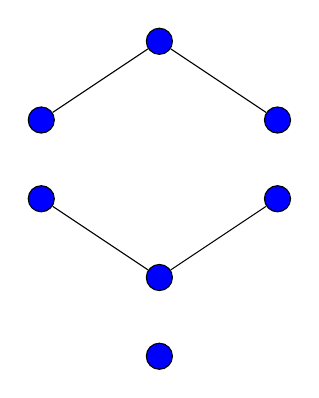
\begin{tikzpicture}[x=1.5cm,y=1cm,every node/.style={draw,solid,shape=circle,fill=blue}]

  % Specification of nodes (position, etc.)
  \node (a0) at (0,0) {};
  \node (b0) at (-1,-1) {};
  \node (b1) at (1,-1) {};
  \node (g0) at (-1,-2) {};
  \node (g1) at (1,-2) {};
  \node (j) at (0,-3) {};
  \node (c) at (0,-4) {};

  \begin{scope}[-]
    \tikzstyle{every node}=[draw,below]
    \draw[solid] (a0) to (b0);
    \draw[solid] (a0) to (b1);
    \draw[solid] (g0) to (j);
    \draw[solid] (g1) to (j);
  \end{scope}

\end{tikzpicture}
 };
    \node[scale=0.4] (state1a) at (4, 1.5) { 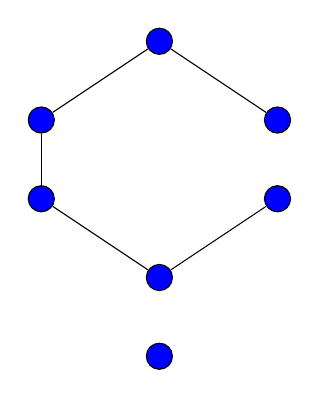
\begin{tikzpicture}[x=1.5cm,y=1cm,every node/.style={draw,shape=circle,fill=blue}]

  % Specification of nodes (position, etc.)
  \node (a0) at (0,0) {};
  \node (b0) at (-1,-1) {};
  \node (b1) at (1,-1) {};
  \node (g0) at (-1,-2) {};
  \node (g1) at (1,-2) {};
  \node (j) at (0,-3) {};
  \node (c) at (0,-4) {};

  \begin{scope}[-]
    \tikzstyle{every node}=[draw=none,below]
    \draw (a0) to (b0);
    \draw (a0) to (b1);
    \draw (b0) to (g0);
    \draw (g0) to (j);
    \draw (g1) to (j);
  \end{scope}

\end{tikzpicture}
 };
    \node[scale=0.4] (state1b) at (3, -1) { 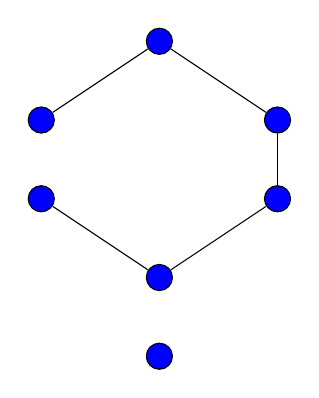
\begin{tikzpicture}[x=1.5cm,y=1cm,every node/.style={draw,shape=circle,fill=blue}]

  % Specification of nodes (position, etc.)
  \node (a0) at (0,0) {};
  \node (b0) at (-1,-1) {};
  \node (b1) at (1,-1) {};
  \node (g0) at (-1,-2) {};
  \node (g1) at (1,-2) {};
  \node (j) at (0,-3) {};
  \node (c) at (0,-4) {};

  \begin{scope}[-]
    \tikzstyle{every node}=[draw=none,below]
    \draw (a0) to (b0);
    \draw (a0) to (b1);
    \draw (b1) to (g1);
    \draw (g0) to (j);
    \draw (g1) to (j);
  \end{scope}

\end{tikzpicture}
 };
    \node[scale=0.4] (state2) at (4, -1) { 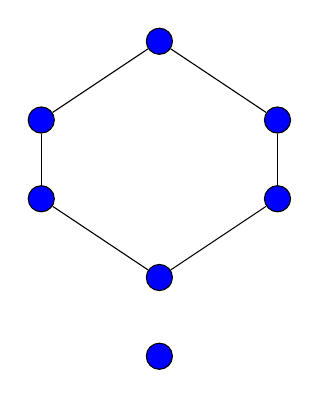
\begin{tikzpicture}[x=1.5cm,y=1cm,every node/.style={draw,shape=circle,fill=blue}]

  % Specification of nodes (position, etc.)
  \node (a0) at (0,0) {};
  \node (b0) at (-1,-1) {};
  \node (b1) at (1,-1) {};
  \node (g0) at (-1,-2) {};
  \node (g1) at (1,-2) {};
  \node (j) at (0,-3) {};
  \node (c) at (0,-4) {};

  \begin{scope}[-]
    \tikzstyle{every node}=[draw=none,below]
    \draw (a0) to (b0);
    \draw (a0) to (b1);
    \draw (b0) to (g0);
    \draw (b1) to (g1);
    \draw (g0) to (j);
    \draw (g1) to (j);
  \end{scope}

\end{tikzpicture}
 };
    \node[scale=0.4, rectangle, draw, dashed, rounded corners] (state3) at (4, -3.5) { 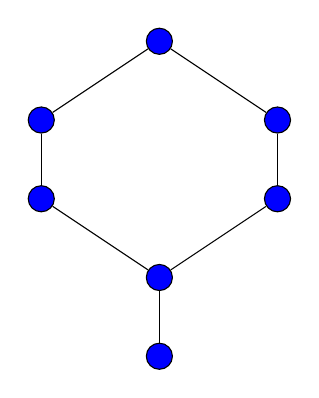
\begin{tikzpicture}[x=1.5cm,y=1cm,every node/.style={draw,solid,shape=circle,fill=blue}]

  % Specification of nodes (position, etc.)
  \node (a0) at (0,0) {};
  \node (b0) at (-1,-1) {};
  \node (b1) at (1,-1) {};
  \node (g0) at (-1,-2) {};
  \node (g1) at (1,-2) {};
  \node (j) at (0,-3) {};
  \node (c) at (0,-4) {};

  \begin{scope}[-]
    \tikzstyle{every node}=[draw=none,below]
    \draw[solid] (a0) to (b0);
    \draw[solid] (a0) to (b1);
    \draw[solid] (b0) to (g0);
    \draw[solid] (b1) to (g1);
    \draw[solid] (g0) to (j);
    \draw[solid] (g1) to (j);
    \draw[solid] (j) to (c);
  \end{scope}

\end{tikzpicture}
 };
    \node (expanded3) at (1, -6) { \begin{tikzpicture}[x=2.4cm, y=1cm, framed, background rectangle/.style={draw=black,dashed, rounded corners}] 

  % Specification of nodes (position, etc.)
  \node (a0) at (0,0) { $\adj{\alpha_L(x)\alpha_{L'}(x)}$ };
  \node (b0) at (-1,-1) { $\enf{\beta_L(G: x)}_{A, C}$ };
  \node (b1) at (1,-1) { $\enf{\beta_{L'}(G': x)}_{B, C}$ };
  \node (g0) at (-1,-2) { $\enf{\gamma_{G, J}(\rchi, A, C)}_{A, C}$ };
  \node (g1) at (1,-2) { $\enf{\gamma_{G', J}(\rchi, B, C)}_{B, C}$ };
  \node (j) at (0,-3) { $\enf{\beta_J(\rchi: x, C: x)}_{A,B,C}$ };
  \node (c) at (0,-4) { $\enf{\beta_\rchi(A: a, B: b)}_{A,B}$ };

  \begin{scope}[-]
    \tikzstyle{every node}=[draw=none,below]
    \draw (a0) to (b0);
    \draw (a0) to (b1);
    \draw (b0) to (g0);
    \draw (b1) to (g1);
    \draw (g0) to (j);
    \draw (g1) to (j);
    \draw (j) to (c);
  \end{scope}

\end{tikzpicture}
 };

    \begin{scope}[ultra thick]
      \tikzstyle{every node}=[below]
      \draw[-{Latex[length=3mm,width=4mm]}] (state0) edge (state1a)
                (state0) edge (state1b)
                (state1a) edge (state2)
                (state1b) edge (state2)
                (state2) edge (state3);
    \end{scope}
  \end{tikzpicture}
  \caption{Ledger channels, $x = a + b$}
  \label{fig:modes}
\end{figure} 

  \caption{Opening a virtual channel}
  \label{fig:virtual-channel-opening}
\end{figure}

\begin{tikzpicture}[x=4cm, y=0.7cm]
  \node at (0, 0) {
    \begin{tikzpicture}[x=.8cm]
      \node[sqadj] (a0) at (-1,0) {};
      \node[sqadj] (a1) at (1,0) {};
      \node[circAI] (b0) at (-1,-1) {};
      \node[circBI] (b1) at (1,-1) {};
      \node[guarAI] (g0) at (-1,-2) {};
      \node[guarBI] (g1) at (1,-2) {};
      \node[circABI] (j) at (0,-3) {};
      \node[circAB] (c) at (0,-4) {};

      \begin{scope}[-]
        \tikzstyle{every node}=[draw,below]
        \draw[solid] (a0) to (b0);
        \draw[solid] (a1) to (b1);
        \draw[solid] (g0) to (j);
        \draw[solid] (g1) to (j);
      \end{scope}
    \end{tikzpicture}
  };

  \node at (1, 0) {
    \begin{tikzpicture}[x=0.8cm]
      \node[sqadj] (a0) at (-1,0) {};
      \node[sqadj] (a1) at (1,0) {};
      \node[circAI] (b0) at (-1,-1) {};
      \node[circBI] (b1) at (1,-1) {};
      \node[guarAI] (g0) at (-1,-2) {};
      \node[guarBI] (g1) at (1,-2) {};
      \node[circABI] (j) at (0,-3) {};
      \node[circAB] (c) at (0,-4) {};

      \begin{scope}[-]
        \tikzstyle{every node}=[draw,below]
        \draw[solid] (a0) to (b0);
        \draw[solid] (a1) to (b1);
        \draw[solid] (b0) to (g0);
        \draw[solid] (g0) to (j);
        \draw[solid] (g1) to (j);
      \end{scope}
    \end{tikzpicture}
  };

  \node at (2, 0) {
    \begin{tikzpicture}[x=0.8cm]
      \node[sqadj] (a0) at (-1,0) {};
      \node[sqadj] (a1) at (1,0) {};
      \node[circAI] (b0) at (-1,-1) {};
      \node[circBI] (b1) at (1,-1) {};
      \node[guarAI] (g0) at (-1,-2) {};
      \node[guarBI] (g1) at (1,-2) {};
      \node[circABI] (j) at (0,-3) {};
      \node[circAB] (c) at (0,-4) {};

      \begin{scope}[-]
        \tikzstyle{every node}=[draw,below]
        \draw[solid] (a0) to (b0);
        \draw[solid] (a1) to (b1);
        \draw[solid] (b0) to (g0);
        \draw[solid] (b1) to (g1);
        \draw[solid] (g0) to (j);
        \draw[solid] (g1) to (j);
      \end{scope}
    \end{tikzpicture}
  };

  \node at (3, 0) {
    \begin{tikzpicture}[x=0.8cm]
      \node[sqadj] (a0) at (-1,0) {};
      \node[sqadj] (a1) at (1,0) {};
      \node[circAI] (b0) at (-1,-1) {};
      \node[circBI] (b1) at (1,-1) {};
      \node[guarAI] (g0) at (-1,-2) {};
      \node[guarBI] (g1) at (1,-2) {};
      \node[circABI] (j) at (0,-3) {};
      \node[circAB] (c) at (0,-4) {};

      \begin{scope}[-]
        \tikzstyle{every node}=[draw,below]
        \draw[solid] (a0) to (b0);
        \draw[solid] (a1) to (b1);
        \draw[solid] (b0) to (g0);
        \draw[solid] (b1) to (g1);
        \draw[solid] (g0) to (j);
        \draw[solid] (g1) to (j);
        \draw[solid] (j) to (c);
      \end{scope}
    \end{tikzpicture}
  };
\end{tikzpicture}

The same sequence of states, when taken in reverse, can be used to close a virtual channel:
\begin{enumerate}
  \item Participants $A$ and $B$ finalize $\rchi$ by signing a conclusion proof:
  \begin{align}
    \finalizable{\rchi}{\alloc{A:a', B:b'}}{A,B}
  \end{align}
  \item $A$ and $B$ sign an update to $J$ to take account of the outcome of $\rchi$. $I$ will accept this update, provided that their allocation of $x$ coins remains the same:
  \begin{align}
    \finalizable{J}{\alloc{A: a', B:b', I: x}}{A, B, I}
  \end{align}
  \item In either order switch the ledger channels to absorb the outcome of $J$, defunding the guarantor channels in the process:
  \begin{align}
    & \finalizable{L}{\alloc{A: a', I: b'}}{A,I} \\
    & \finalizable{L'}{\alloc{B: b', I: a'}}{B,I}
  \end{align}
  \item The channels $\rchi$, $J$, $G$ and $G'$ are now all defunded, so can be discarded
\end{enumerate}

It is also possible to do top-ups and partial checkouts from a virtual channel.
